\documentclass{article}
\usepackage{graphicx}
\usepackage[utf8x]{inputenc}

\graphicspath{{images/}}

\begin{document}

\begin{titlepage}
	\begin{center}
		\vspace*{1cm}
 
		\Huge
		\textbf{Assignment 2 :: Report}
 
		\vspace{0.5cm}
		\Large
		
 
		\vspace{1.5cm}
		Organization of  Digital Computers Lab\\
		EECS 112L\\
		University of California, Irvine\\
		1 March 2019
 
		\vfill

 
		\vspace{0.8cm}
		\Large 
	          	\textbf{	Team CTRL-C CTRL-V } \\
				Aakif Hussain   63828630 \\
				Prannay Kapur  45621364
 
 
	\end{center}
\end{titlepage}
	\Large
	\section{Block Diagram}
		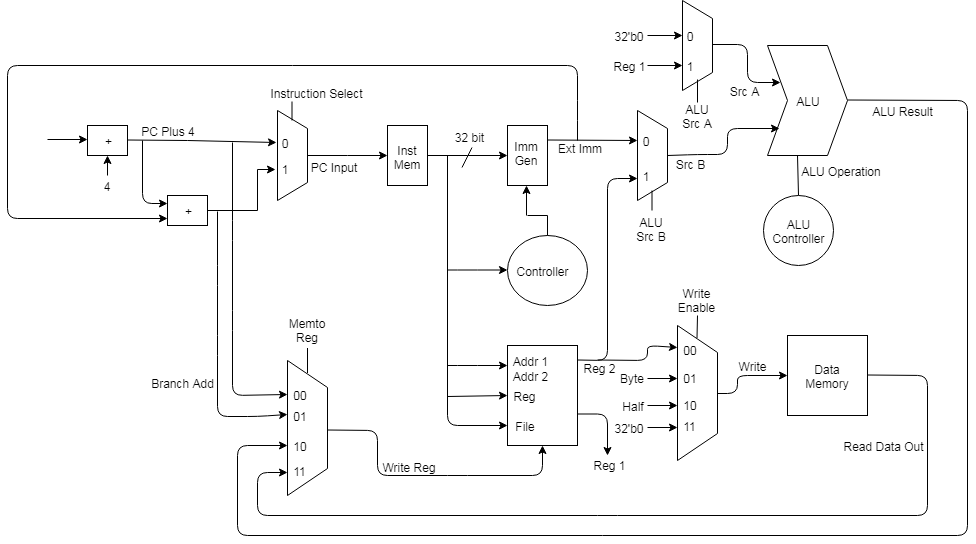
\includegraphics[width=1\textwidth]{block_diagram.png}
		In the original block diagram, the RISC V processor implemented did not support any B type (branching), J type (jumping), or U type (unsigned) instructions.
		Our newly implemented design now features these instructions, and the following changes were made to support them:
			\begin{itemize}\normalsize
				\item For the Immediate Generator, new outputs were included to support reading immediate values from B type, U type, and S type instructions.
				\item For the ALU, the actual instructions were implemented (e.g. AND = input\_1 \& input\_2).
				\item For the Data Memory, the ability to load and store half words and bytes was implemented.
				\item For the Controller, new signal outputs were added to support the different types of U type instructions, the different types of J type instructions,
						and the B type instructions.
				\item For the Datapath, new multiplexers were added to support the new signals from the Controller and actually perform the jumps in the program
						counter given by the B type and J type instructions.
			\end{itemize}			


	\Large
	\section{Module Simulation}
		\large
		\subsection{Screenshots of Waveform}
			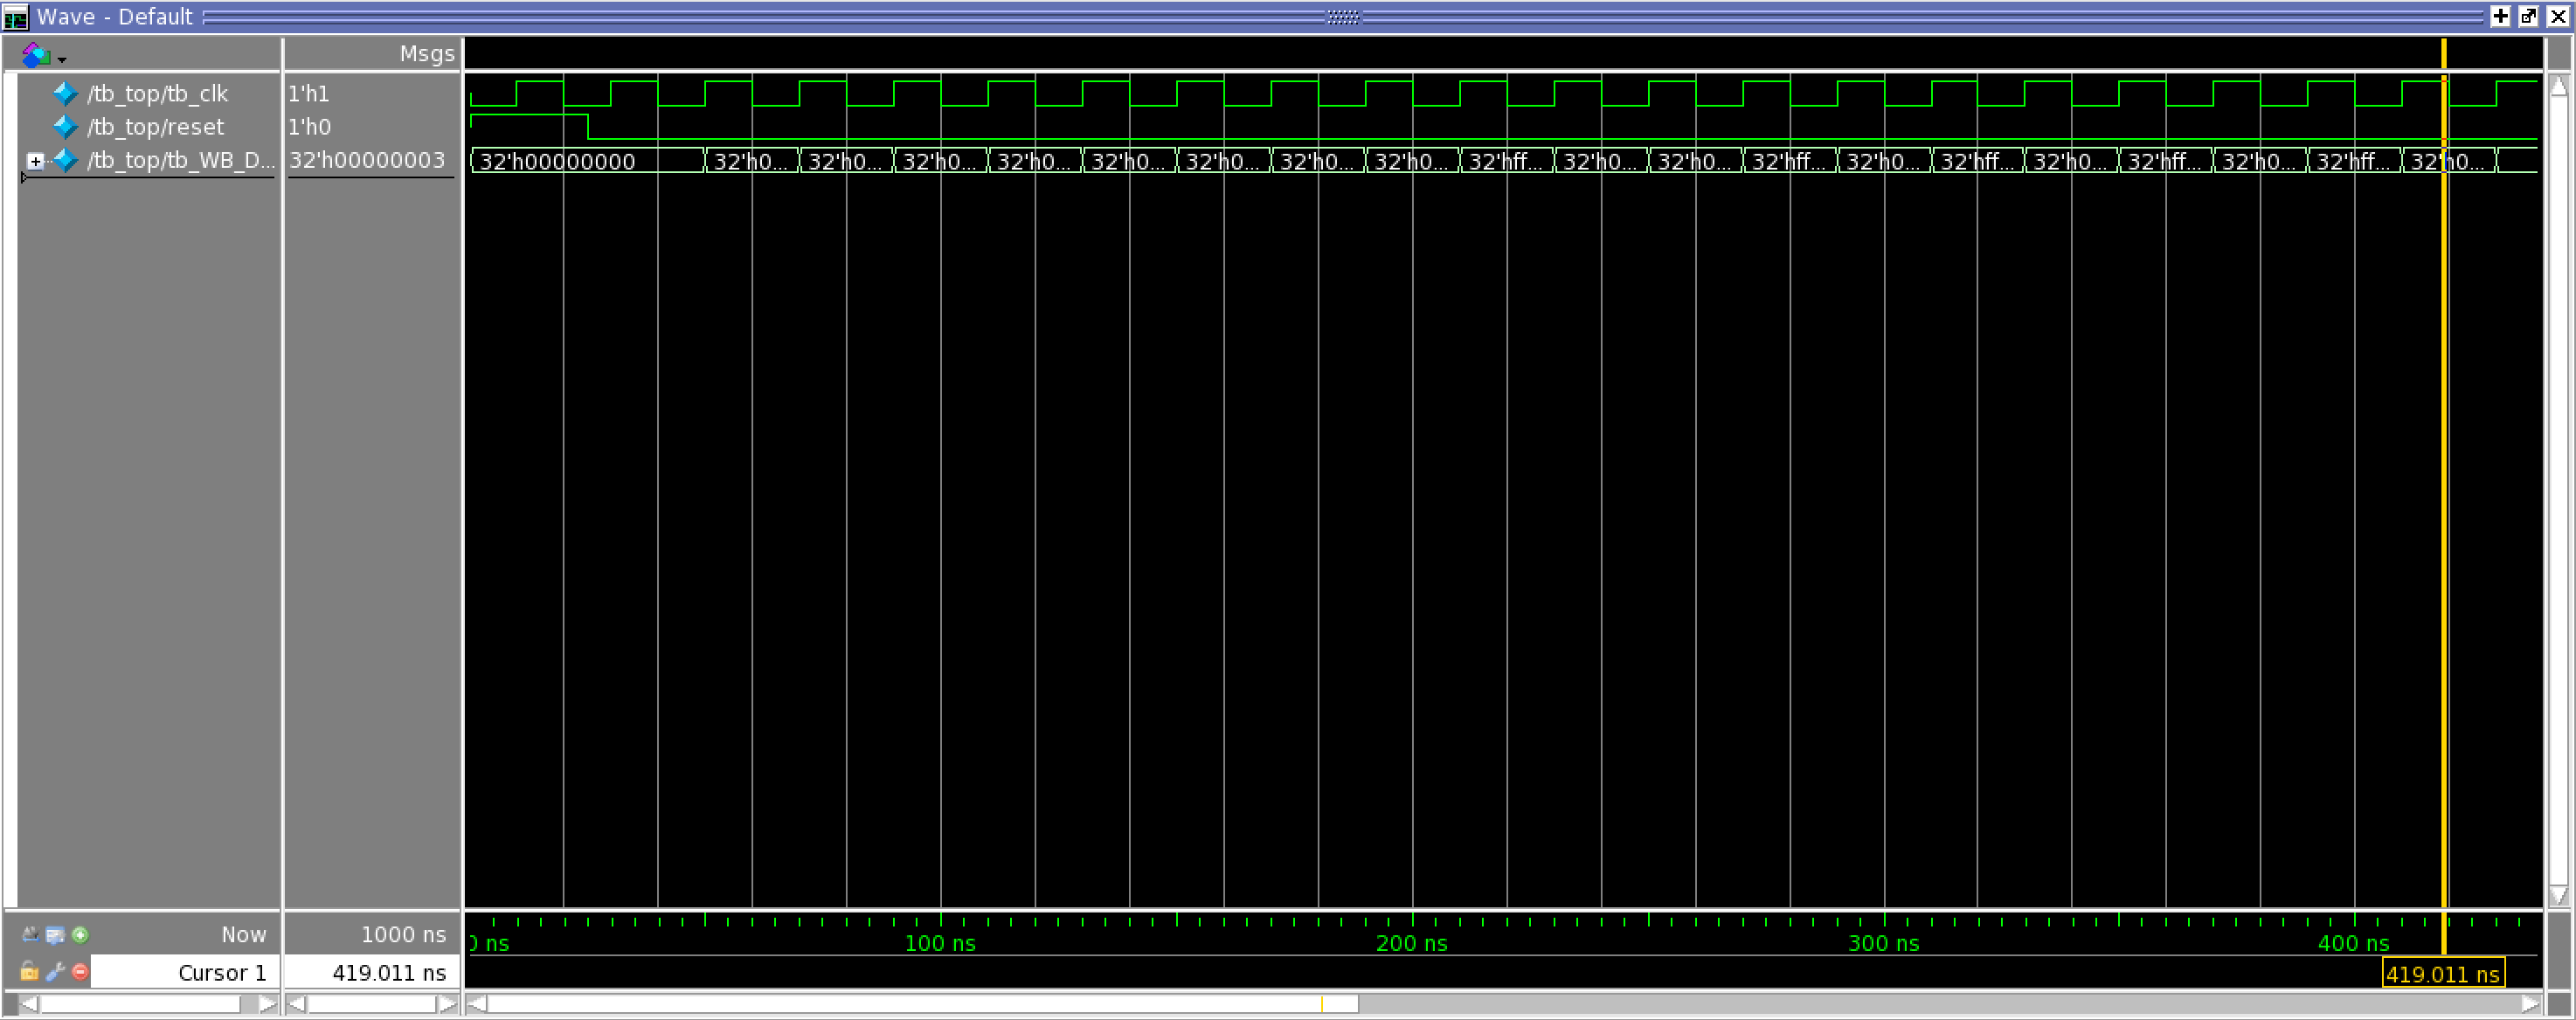
\includegraphics[width=1\textwidth]{waveform1.png}
			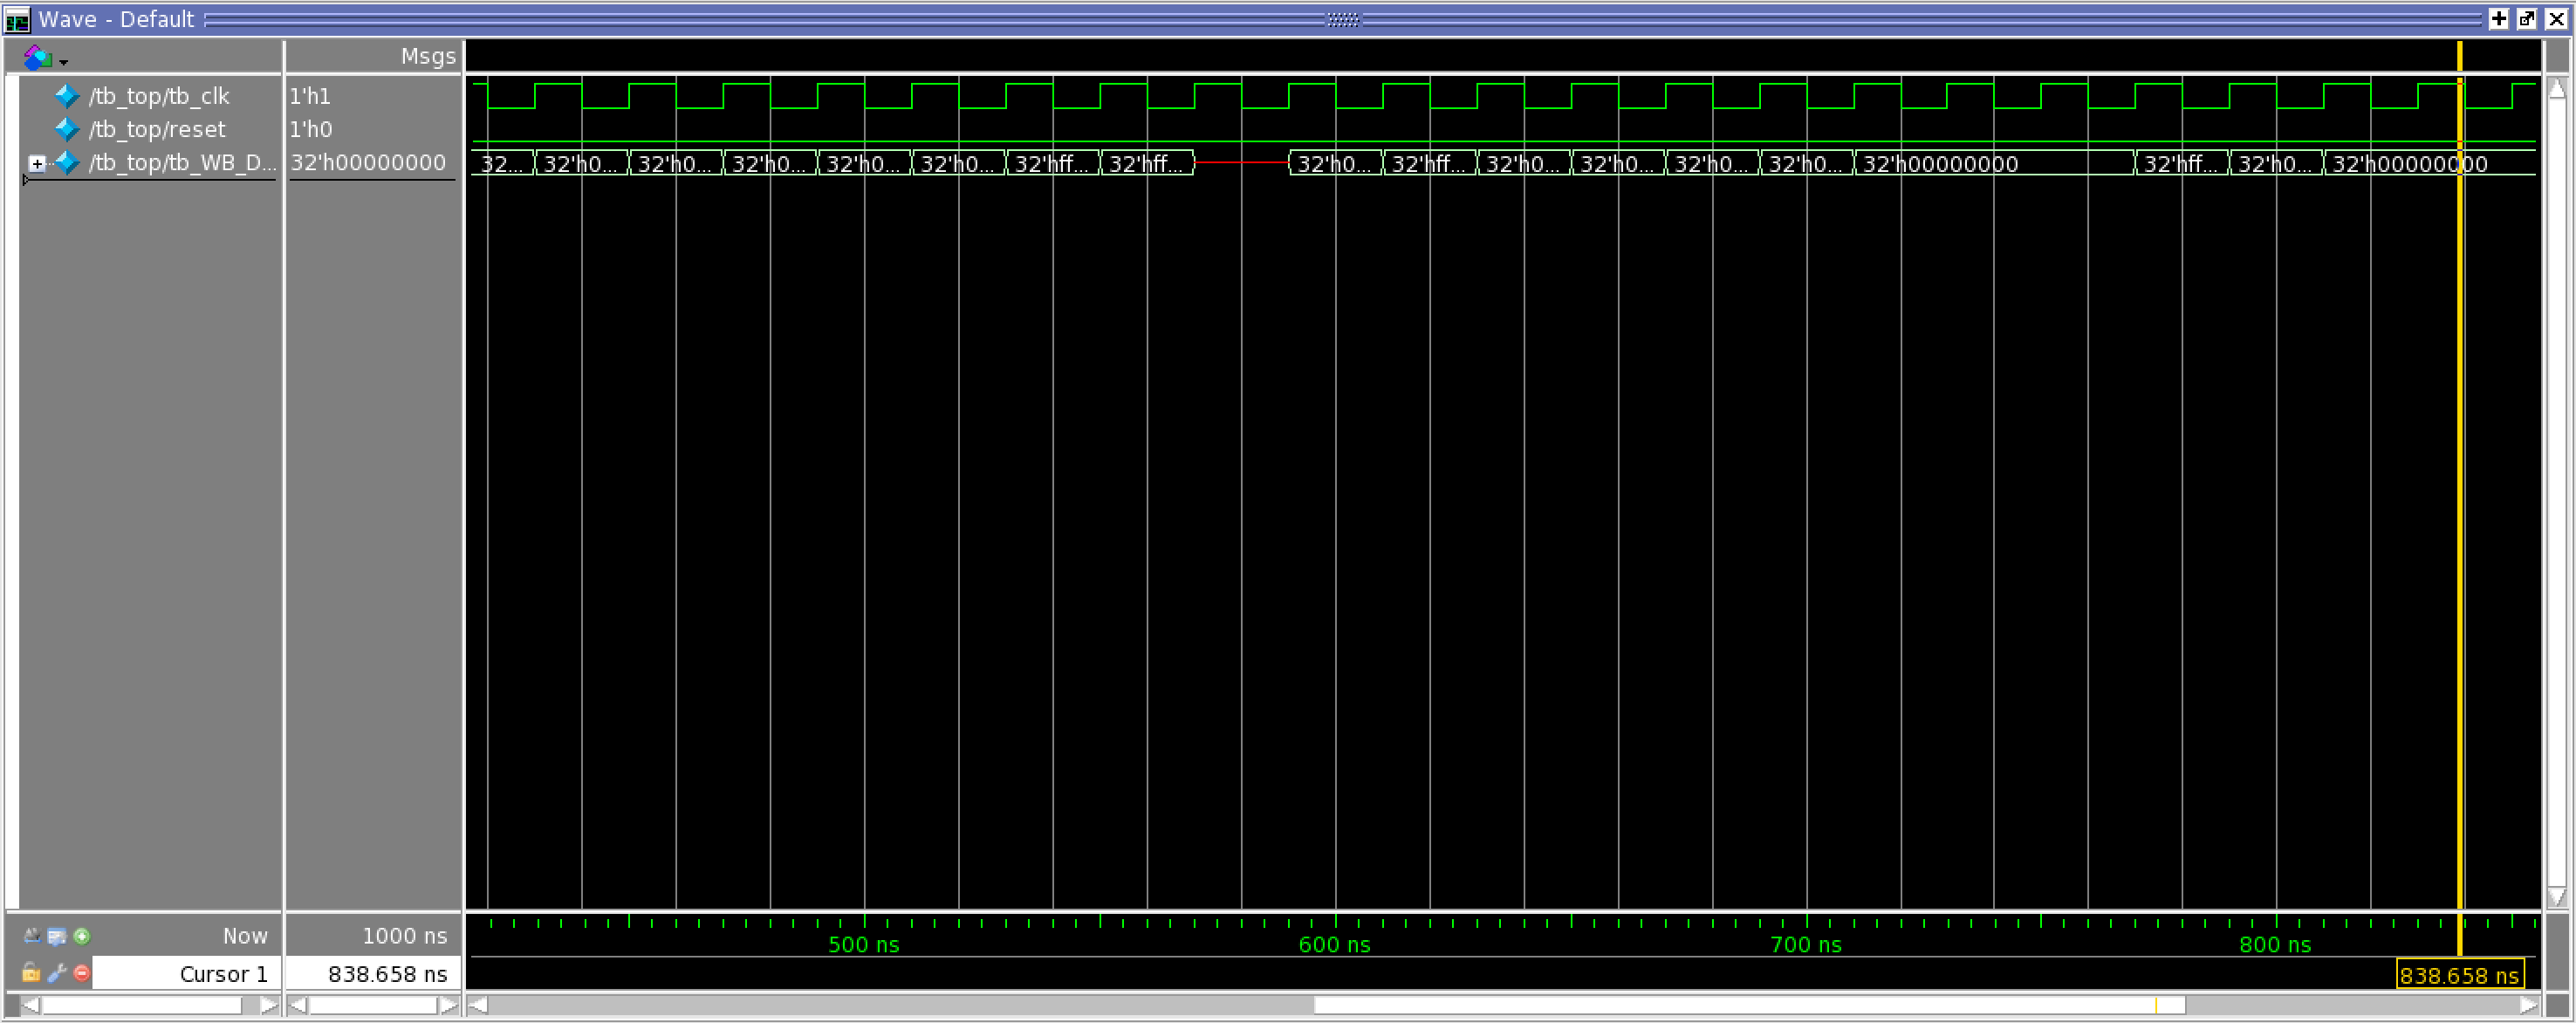
\includegraphics[width=1\textwidth]{waveform2.png}
			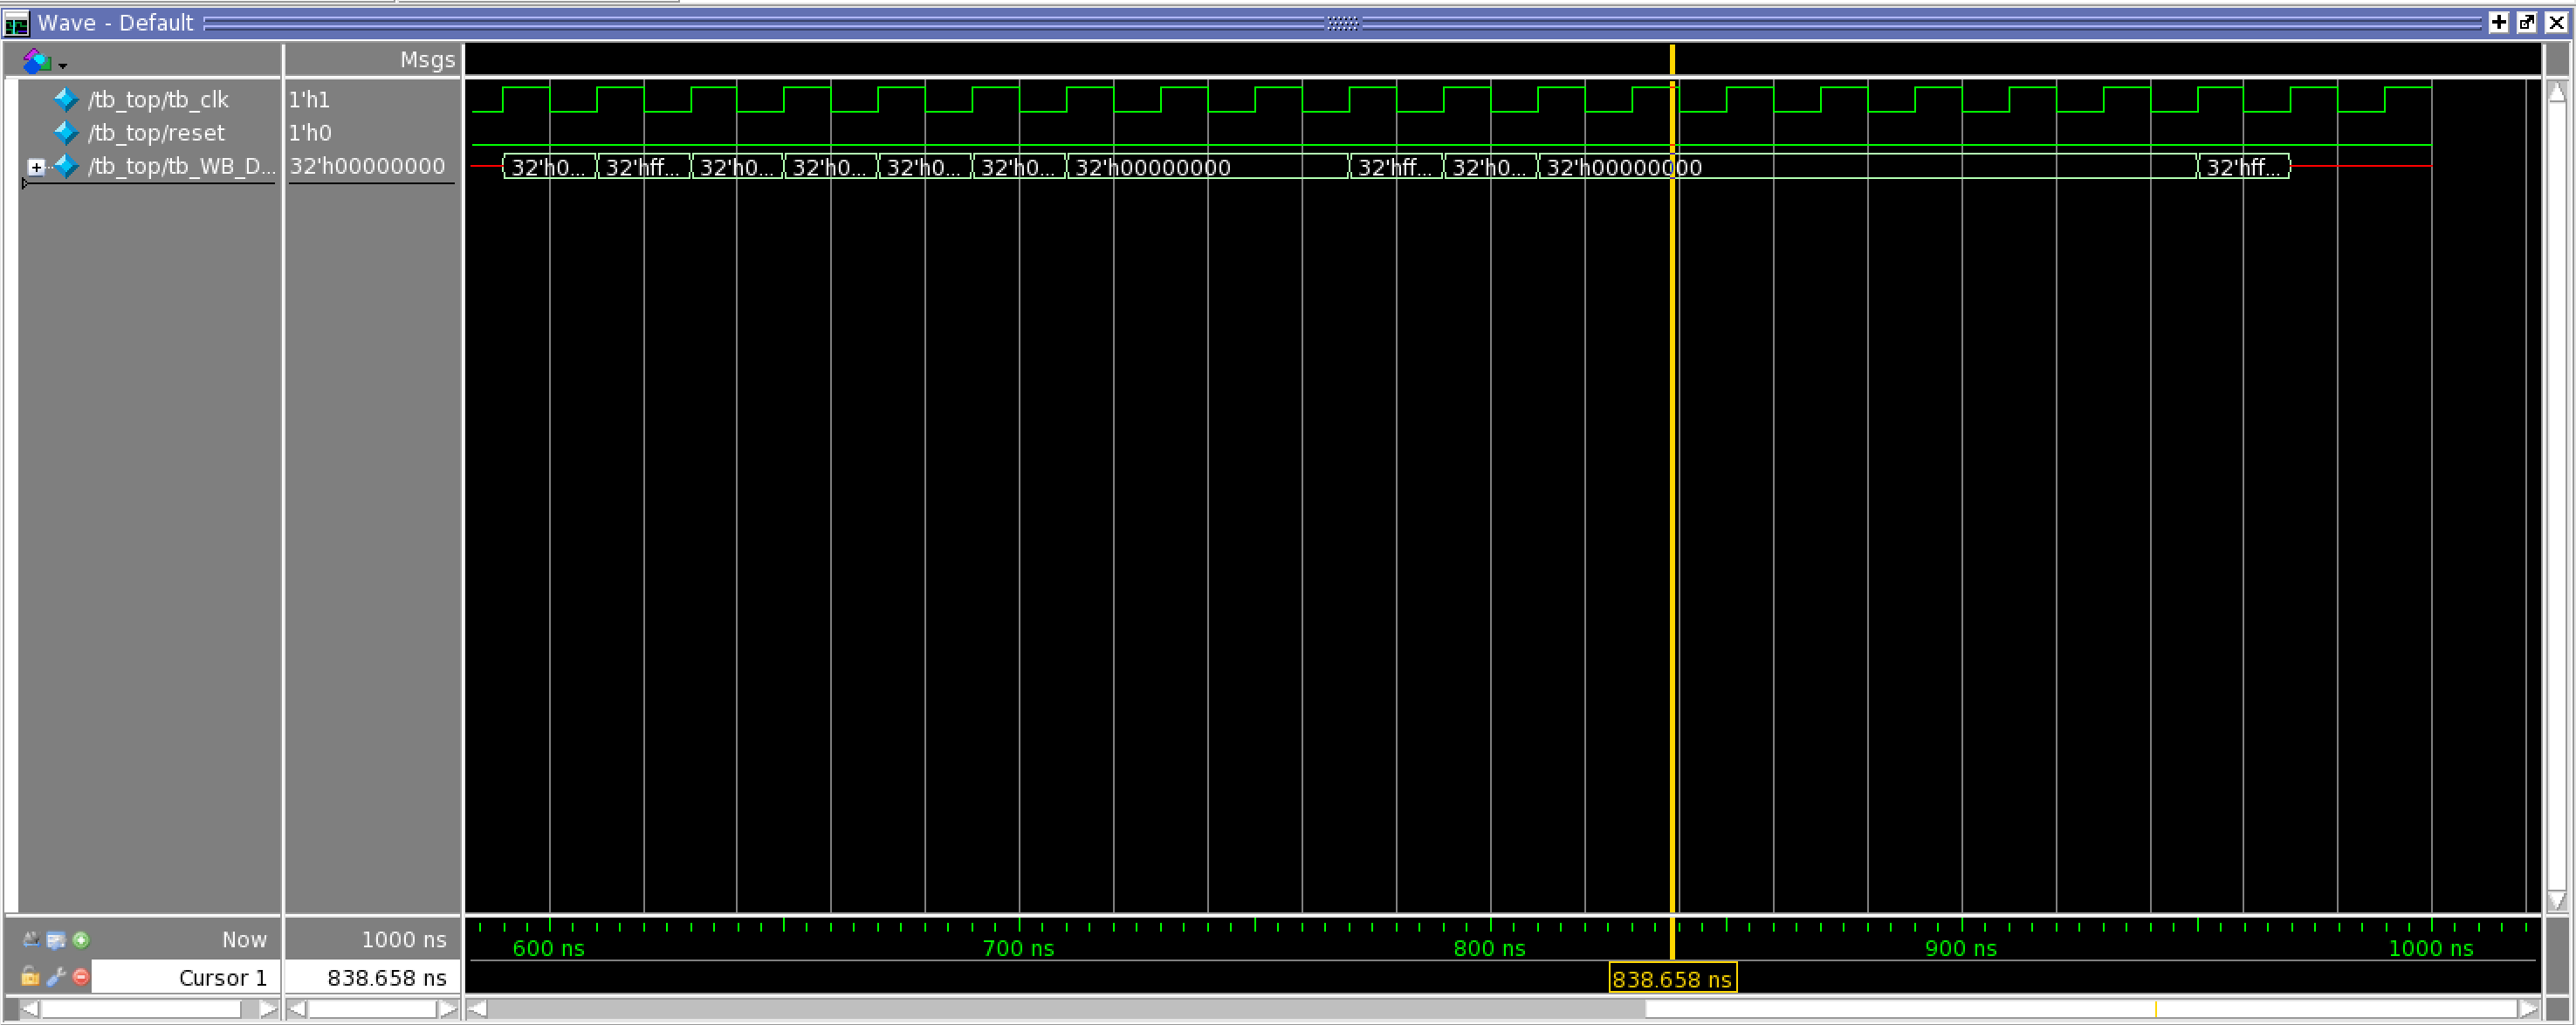
\includegraphics[width=1\textwidth]{waveform3.png}
		\subsection{Complications}
			We faced multiple challenges when adding the new signals to the Datapath from the Controller. One such was an iteration error, because the program
			counter was not able to jump properly in accordance to what the instruction was asking. We faced some issues that were not solvable, such as the
			implementation of a JALR instruction, as for some reason, the 4-1 multiplexer was not able to assign data to the proper output. 
		
	\Large
	\section{Module Synthesis}
		\subsection{Power}
		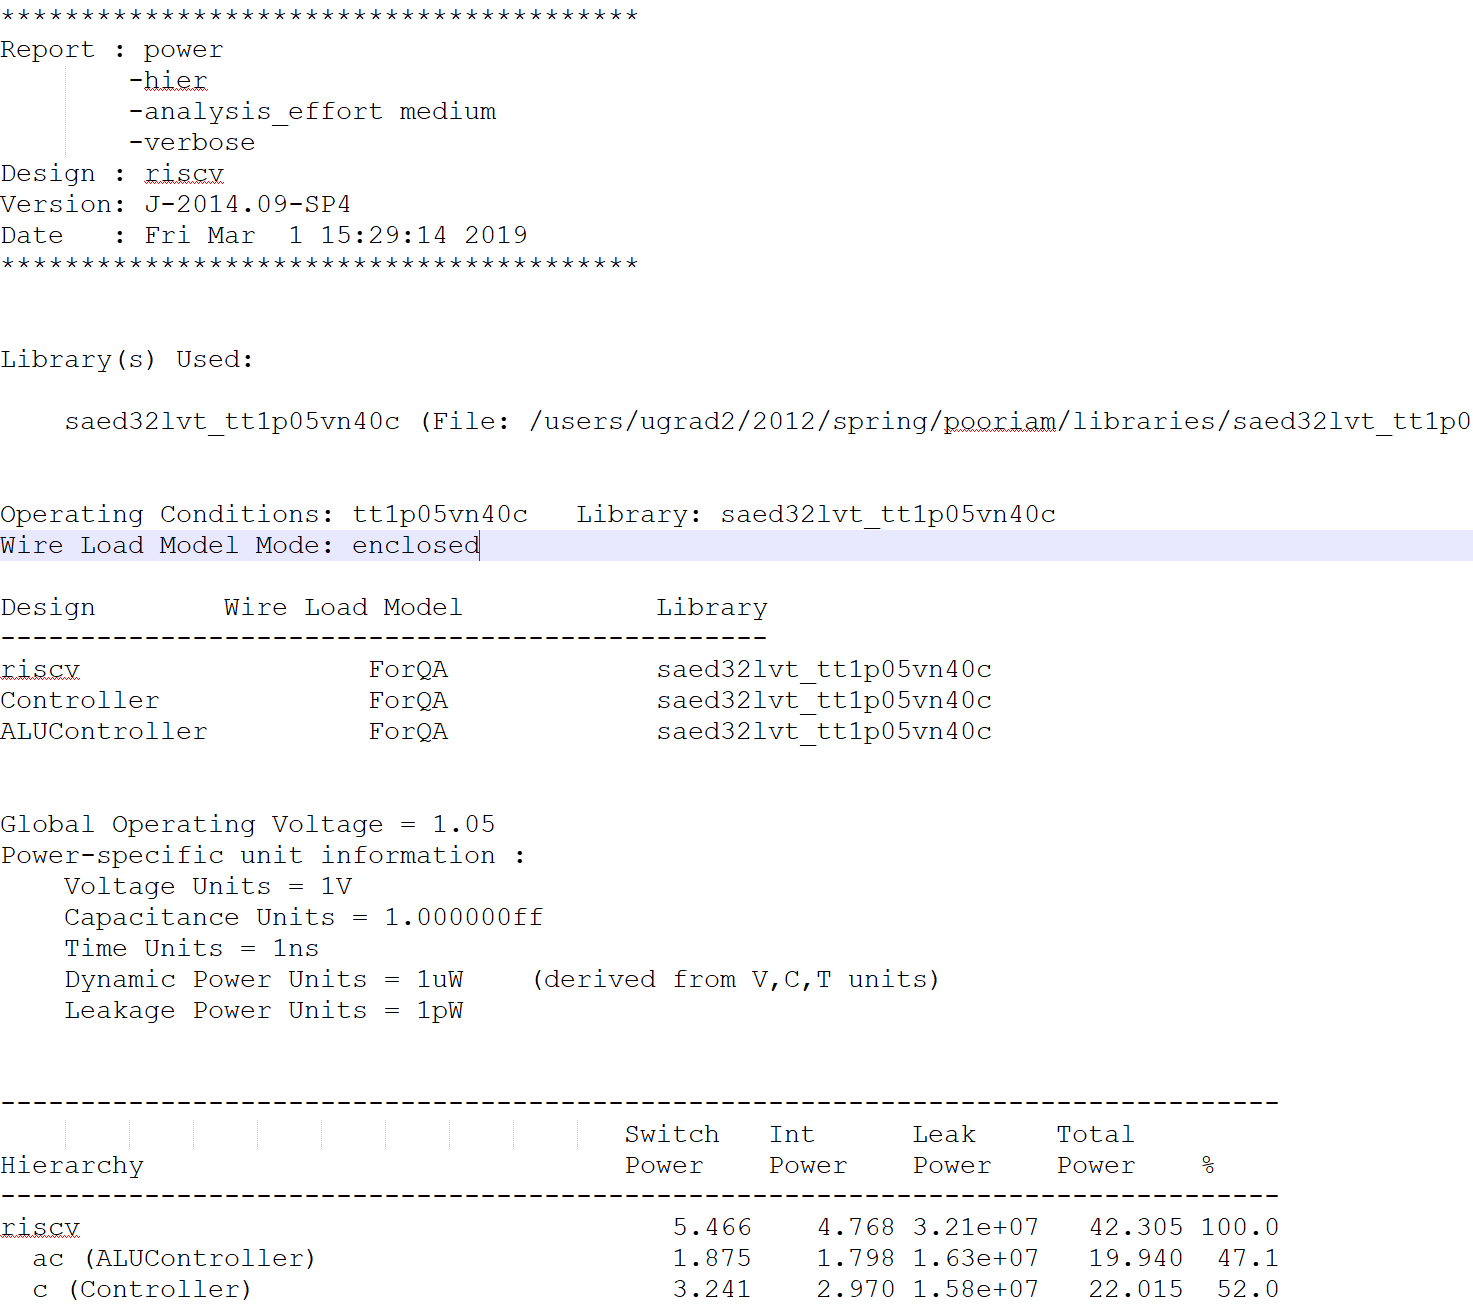
\includegraphics[width=1\textwidth]{power.png}
		\normalsize

		\subsection{Area}
		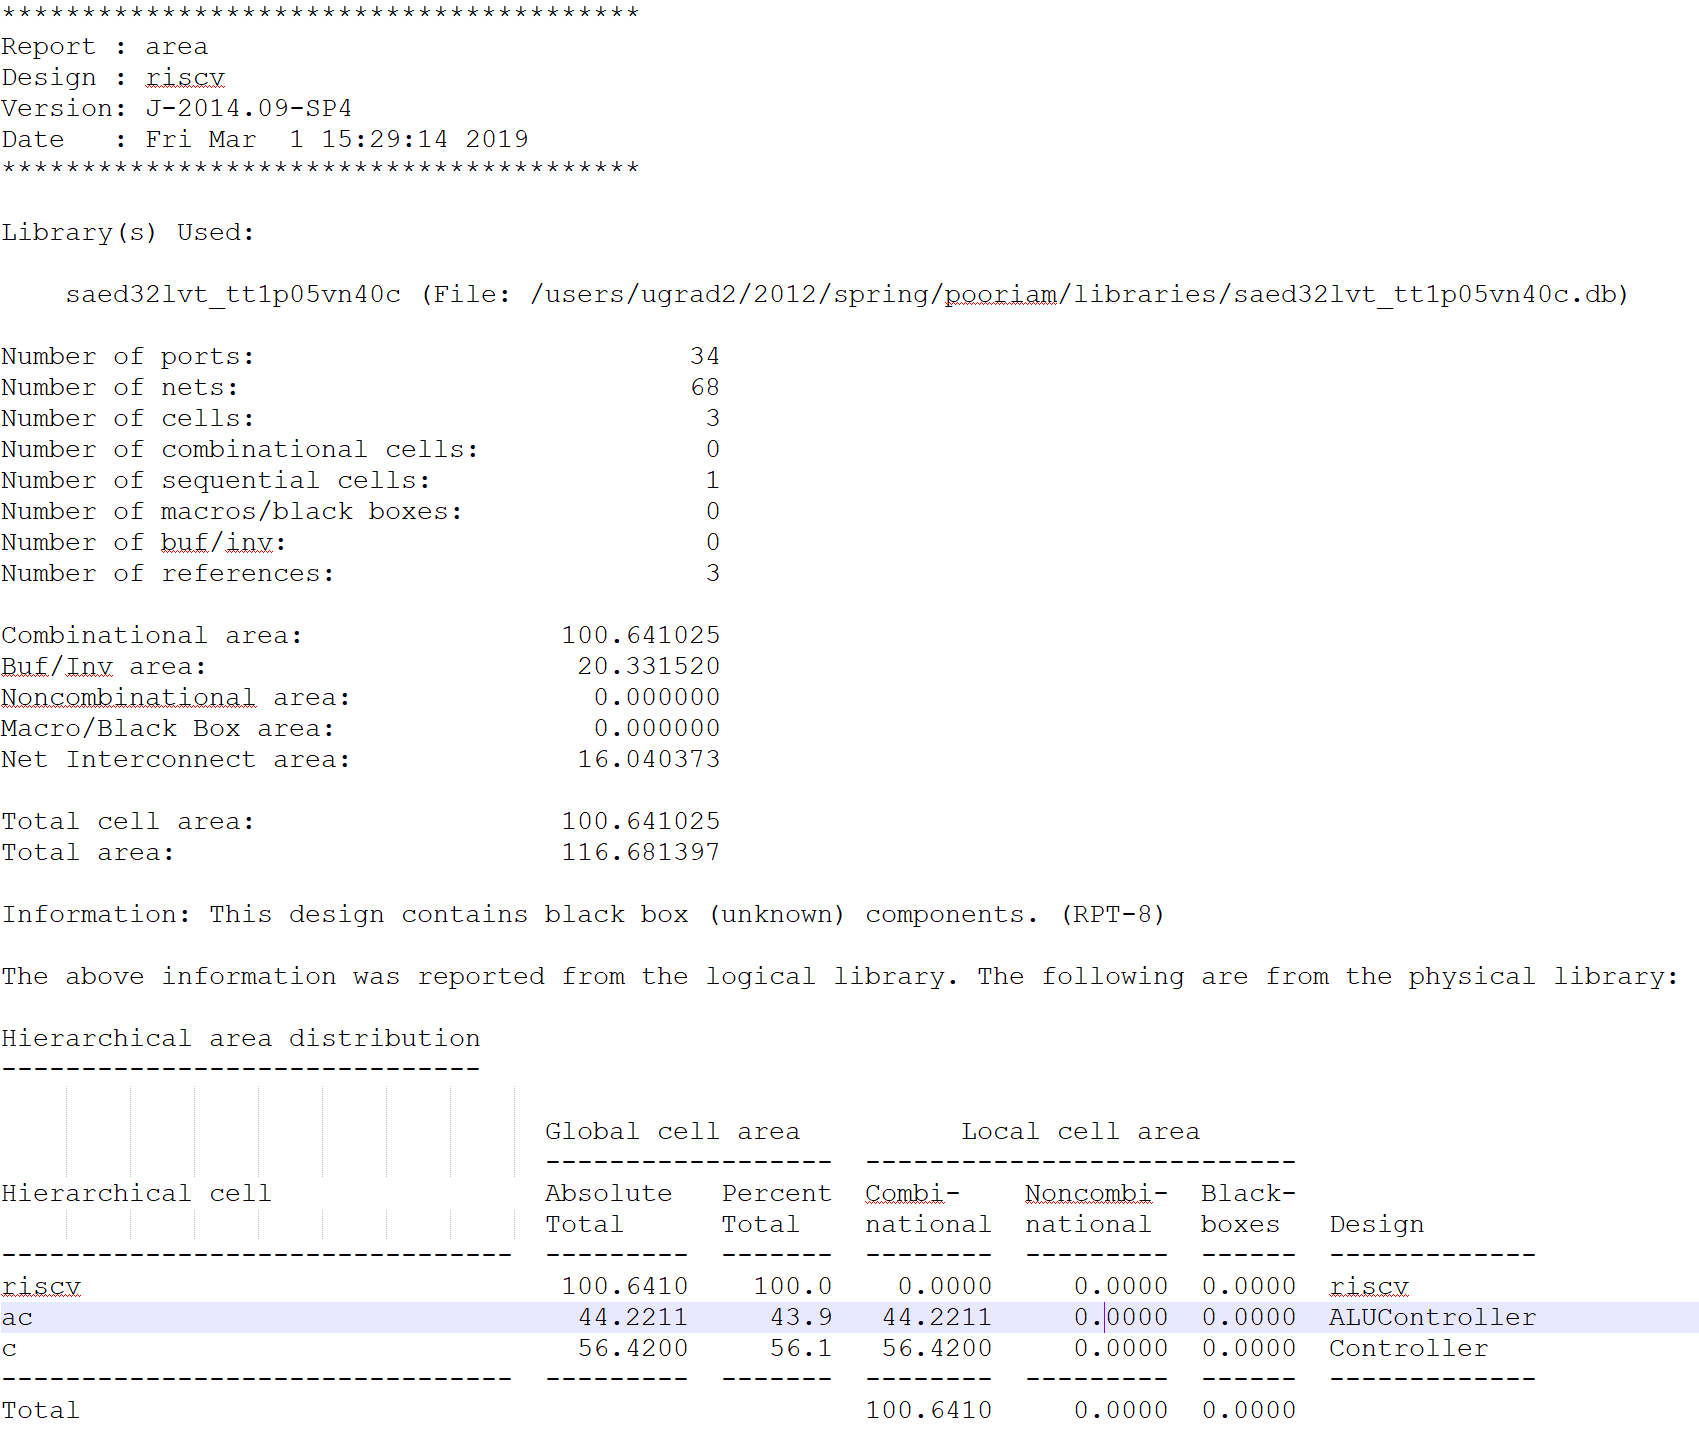
\includegraphics[width=1\textwidth]{area.png}
		\normalsize

		\subsection{Clock Frequency}
		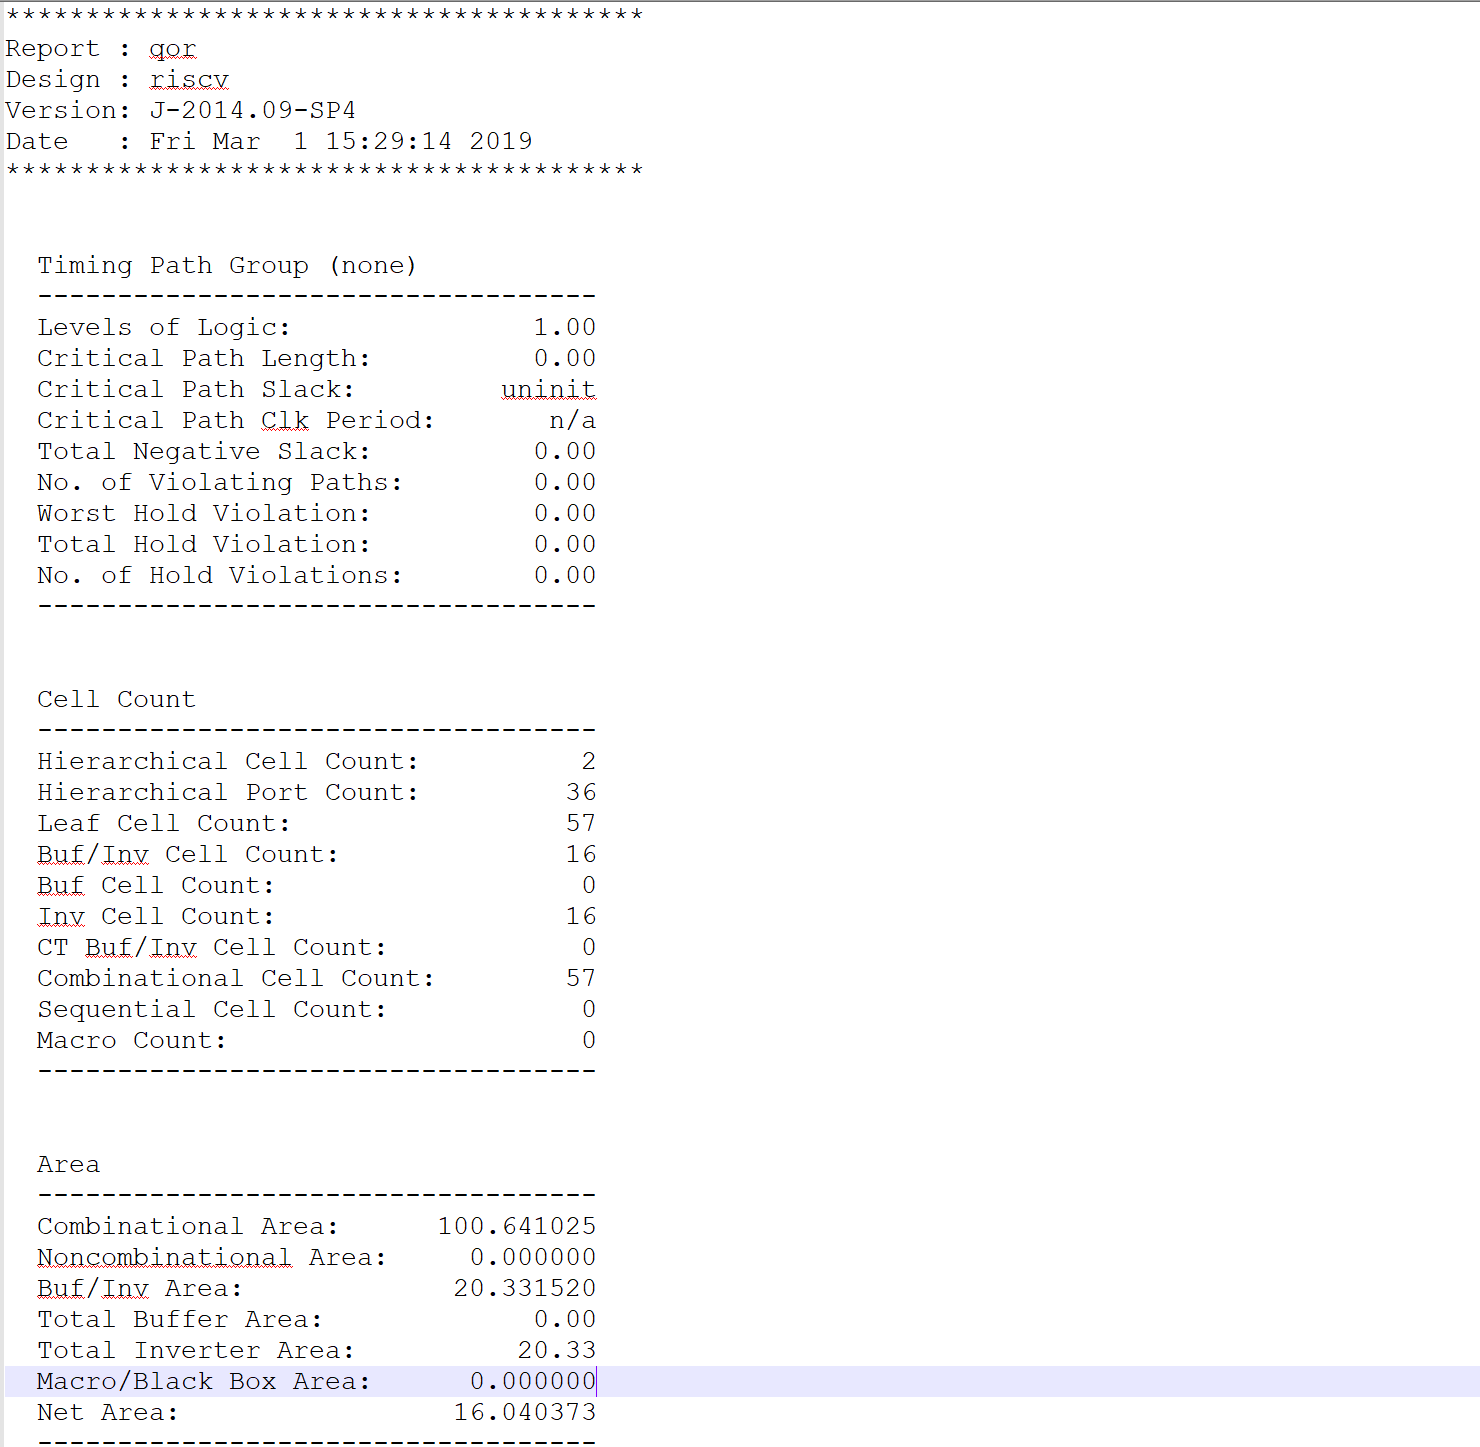
\includegraphics[width=1\textwidth]{frequency.png}
	
\end{document}